\documentclass{ctexart} % 使用 ctex 文档类
\usepackage{amsmath,amssymb,amsthm} % 引入数学公式宏包
\usepackage{mathrsfs} % 引入花体字符宏包
\usepackage{graphicx}
\usepackage{bookmark}
\usepackage{hyperref}
\usepackage{indentfirst}
\usepackage{float}


\newtheorem{theorem}{定理}
\newtheorem{corollary}{推论}

\begin{document}

\title{概率论与数理统计大作业报告:探究本福特定律表述中“自然产生”的定义}
\author{概统冲冲}
\date{\today}
\maketitle

\section{本福特定律阐释与研究目标介绍}

\subsection{本福特定律:一项揭示数字分布规律的数学洞察}

在纷繁复杂的数据海洋中,存在一种普遍且隐秘的数学规律,即本福特定律(Benford’s Law)。该定律揭示了在自然生成的数据集中,数字1作为首位数字出现的频率高达30\%,显著高于基于均匀分布预期的11\%。这一现象不仅令人惊奇,而且呈现出一种非直觉的数学美感。随着首位数字的增大,其出现频率逐渐减少,呈现出一种递减的数学模式。

本福特定律的发现,不仅丰富了理论数学的研究领域,而且在实践层面具有显著的应用价值。特别是在数据真实性检验方面,本福特定律成为了一种有效的分析工具。然而,值得注意的是,本福特定律的应用前提是数据集需覆盖多个数量级,并且数据应当是自然产生的,而非受到人为操纵或选择的产物\cite{wiki_benford}。

\subsection{本福特定律的历史研究}

1881年,天文学家Newcomb即注意到对数表中以1开头的页面明显比其他页面更为破旧。在其论文《关于自然数中不同数字出现频率的注释》中,他基于“数字的对数尾数出现的概率是相等的\footnote{尾数是指将一个数表示为$a\times10^n$的形式时,$a$这个部分,它是一个大于等于1且小于10的实数。}”这一假设,首次计算出了十进制数字中各首位数字出现的概率。\cite{Simon}

\begin{tabular}{|c|p{3cm}|p{6cm}|}
    \hline
    $n$ & $P(n)$ & $P(n)$ 的相对大小   \\
    \hline
    1 & 30.1\% & \rule{4.8cm}{0.2cm} \\ \hline
    2 & 17.6\% & \rule{2.9cm}{0.2cm} \\ \hline
    3 & 12.5\% & \rule{2.1cm}{0.2cm} \\ \hline
    4 & 9.7\% & \rule{1.6cm}{0.2cm} \\ \hline
    5 & 7.9\% & \rule{1.3cm}{0.2cm} \\ \hline
    6 & 6.7\% & \rule{1.1cm}{0.2cm} \\ \hline
    7 & 5.8\% & \rule{0.95cm}{0.2cm} \\ \hline
    8 & 5.1\% & \rule{0.85cm}{0.2cm} \\ \hline
    9 & 4.6\% & \rule{0.75cm}{0.2cm} \\ \hline
\end{tabular}

\vspace{0.5cm}

也就是说,对于一组自然产生的十位数数据集,其首位数字$d$出现的概率$\mathbb{P}(d)$满足以下公式:

\begin{equation}
    \mathbb{P} (d) = \log_{10}(d+1) - \log_{10}(d) , d = 1, 2, \cdots, 9
\end{equation}

更一般地,\footnote{其中$D_k$表示第k位显著数字函数,$d_k$为具体值}
\begin{equation}
    \mathbb{P} (D_1=d_1, D_2=d_2, \cdots, D_k=d_k)=\log_{10}[1+(\sum_{i=1}^{k}d_i\times10^{(k-i)})^{-1}]
\end{equation}

Hill在1995年证明了符合本福特定律的三个等价条件(涉及到的数学符号会在下文解释):\cite{Hilla, Hillb}

\begin{enumerate}
    \item \textbf{尺度不变性}:
    若概率测度 $\mathbb{P} $ 在 $(\mathbb{R}^+,\mathscr{M})$ 上具有尺度不变性,则对于所有 $s>0$ 和 $S\in\mathscr{M}$,有:
    \begin{equation}
        \mathbb{P} (S) = \mathbb{P} (s\times S)
    \end{equation}
    这表明概率测度不随单位或数量级的改变而改变。

    \item \textbf{底数不变性}:
    若概率测度 $\mathbb{P} $ 在 $(\mathbb{R}^+,\mathscr{M})$ 上具有底数不变性,则对于所有 $m\in\mathbb{N}$ 和 $S\in\mathscr{M}$,有:
    \begin{equation}
        \mathbb{P} (S) = \mathbb{P} (S^{1/m})
    \end{equation}
    这意味着概率测度在不同进制系统下保持不变。

    \item \textbf{尾数分布渐近收敛至对数分布}:
    若概率测度 $\mathbb{P} $ 在 $(\mathbb{R}^+,\mathscr{M})$ 上满足:
    \begin{equation}
        \mathbb{P} (\bigcup_{i=-\infty}^{\infty}[1,t)) = \log_{10}(t), \forall t\in[1,10)
    \end{equation}
    则其首位数字分布符合本福特定律。
\end{enumerate}

Hill进一步建立了完整的数学理论框架:\cite{Hilla}

\begin{enumerate}
    \item \textbf{定义自然概率空间}:
    设样本空间 $\Omega = \mathbb{R}^+$,$\sigma$-代数 $\mathscr{M}$ 由尾数函数 ${D_1, D_2, \cdots}$ 生成。
    我们称事件域 $\mathscr{M}$ 为(十进制)尾数 $\sigma$-代数,它是Borel集的子 $\sigma$-代数域:
    
    \begin{equation}
        S\in\mathscr{M} \Leftrightarrow S=\bigcup_{i=-\infty}^{+\infty}B\times10^i,
        \text{其中} B \subseteq [1,10) \text{为Borel集}
    \end{equation}

    $\mathscr{M}$ 具有以下性质:
    \begin{itemize}
        \item 每个非空集合都是无限的,在 $0$ 和 $+\infty$ 处有聚点
        \item 具有尺度不变性:若 $S\in \mathscr{M}$,则 $sS\in \mathscr{M}$ 对于所有 $s>0$ 成立
        \item 具有底数不变性:若 $S\in \mathscr{M}$,则 $S^{1/m}\in \mathscr{M}$ 对于所有 $m\in \mathbb{N}$ 成立
        \item 具有自相似性:若 $S\in \mathscr{M}$,则 $\forall m\in \mathbb{N}^+$,有 $10^{m}S=S$
    \end{itemize}

    \item \textbf{随机概率测度与期望分布测度}:
    随机概率测度(r.p.m.)$\mathbb{M}$是一个从Borel概率测度中取值的随机向量\cite{Kallenberg}。
    r.p.m.$\mathbb{M}$的期望分布测度$\mathbf{E}\mathbb{M}$定义为:
    \begin{equation}
        (\mathbf{E}\mathbb{M})(B) = E(\mathbb{M}(B)), \forall \text{ Borel } B\subset \mathbb{R}
    \end{equation}

    \item \textbf{显著数字的极限定律}:
    Hill证明了以下命题相互等价:
    \begin{enumerate}
        \item  $\mathbb{M}$ 的期望分布测度 $\mathbf{E}\mathbb{M}$ 具有尺度不变性
        \item  $\mathbf{E}\mathbb{M}$ 具有底数不变性且是原子不可分的
        \item  对于所有 $t \in [1, 10]$,$\mathbf{E}[\mathbb{M}(\bigcup_{i=-\infty}^{\infty}[1, t))] = \log_{10} t$
        \item  每个 $\mathbb{M}$-随机样本具有尺度无偏的尾数频率
        \item  $\mathbf{E}\mathbb{M}$ 是原子不可分的,且每个 $\mathbb{M}$-随机样本具有基数无偏的尾数频率
        \item  对于所有 $t \in [1, 10]$,对于每个 $\mathbb{M}$-随机样本 $X_1, X_2, \ldots$,有
            \begin{equation}
                \lim_{n\to\infty} n^{-1} \left\vert \{ i < n : F_\mathbb{M}(X_i) \in [1, t) \} \right\vert = \log_{10} t
            \end{equation}
            几乎必然成立
    \end{enumerate}
    \item \textbf{一个解释}:\\
    为了更好地理解Hill的理论,我们可以从尺度不变性出发,尝试推导本福特定律的基本公式:\\
        首先,令$F_\mathbb{M}(t)=\mathbb{M}(\bigcup_{i=-\infty}^{\infty}[1,t)\times10^i)$表示首位数字不超过$t$的概率,即$\mathbb{P}(1\leq D_1 \leq t), t\in[1,10)$\\
        对任意$s>0$,考虑将数据放大$s$倍后的分布函数:\\
        $F_{s\times\mathbb{M}}(t)=\mathbb{P}_{\mathbb{M}}(s \leq D_1 \leq s\times t)=F_{\mathbb{M}}(s\times t) - F_{\mathbb{M}}(s)$\\
        由$\mathbb{M}$的期望分布测度$\mathbf{E}\mathbb{M}$具有尺度不变性,可知对任意Borel集$B\subset \mathbb{R}$,有:\\
        $E(\mathbb{M}(B))=E(s\times\mathbb{M}(B))$\\
        这等价于$F_\mathbb{M}(x)=F_{s\times\mathbb{M}}(x)$. 结合上式可得:\\
        $F_{\mathbb{M}}(t)=F_{\mathbb{M}}(s\times t)-F_{\mathbb{M}}(s)$\\
        再考虑边界条件,我们得到以下函数方程组:
        \begin{equation}
            \begin{cases}
                F_{\mathbb{M}}(t)+F_{\mathbb{M}}(s)=F_{\mathbb{M}}(s\times t)\\
                F_{\mathbb{M}}(1)=0\\
                F_{\mathbb{M}}(10)=1\\
            \end{cases}
        \end{equation}
        可以证明,满足上述条件的唯一连续函数是$F_{\mathbb{M}}(t)=\log_{10}t$\\
        因此,首位数字为$d$的概率为:\\
        $\mathbb{P}(d)=F_{\mathbb{M}}(d+1)-F_{\mathbb{M}}(d)=\log_{10}(d+1)-\log_{10}(d), d=1,2,\cdots,9$
\end{enumerate}
总结而言,我们首先观察到,符合本福特定律的数据展现出尺度不变性,即对于任意 $s > 0$,数据集 $K_1 = \{X_1, X_2, \cdots, X_n\}$ 与其尺度变换后的数据集 $K_2 = \{s \times X_1, s \times X_2, \cdots, s \times X_n\}$ 在 $\mathbb{M}$ 意义下的分布差异微乎其微。

\subsection{本福特定律的应用}
1972年,Hal Varian提出这个定律来用作检查支持某些公共计划的经济数据有否欺瞒之处。1992年,Mark J. Nigrini便在其博士论文"The Detection of Income Tax Evasion Through an Analysis of Digital Frequencies."(Ph.D. thesis. Cincinnati, OH: University of Cincinnati, 1992.)提出以它检查是否有伪帐。\cite{wiki_benford}

推而广之,它能用于在会计学、金融甚至选举中出现的数据。比如本福德定律曾被用作2009 年伊朗选举舞弊的潜在证据 。\cite{Iran}

\subsection{研究目标}

尽管本福特定律的证明已经相当明确,但在判断某个数据样本与本福特定律的契合度方面,仍缺乏具体的条件。为此,我们将从理论层面探讨随机变量符合本福特定律所需满足的条件,并尝试找到一个易于计算且能够模糊地反映数据样本与本福特定律接近程度的特征指标。从而探究出本福特定律中“自然产生”的定义。

\section{研究方法与研究对象}

\subsection{研究方法}

本研究主要采用以下方法:

\begin{enumerate}
    \item \textbf{理论分析}:
    \begin{itemize}
        \item 研究连续型随机变量符合本福特定律的数学条件
        \item 分析概率分布的基本特征与本福特定律的关系
    \end{itemize}

    \item \textbf{数值模拟}:
    \begin{itemize}
        \item 使用Monte Carlo方法生成不同参数的随机样本
        \item 实现Python程序验证理论推导结果
    \end{itemize}

    \item \textbf{实证研究}:
    \begin{itemize}
        \item 收集并分析真实数据集
        \item 计算关键统计量以验证数据与本福特定律的契合度
    \end{itemize}
\end{enumerate}
\subsection{研究对象}

研究对象为正实数范围内的多数量级上的数据序列,特别是:
\begin{itemize}
    \item 连续型随机变量及其分布
    \item 实际数据集(如天体数据、金融数据等)
    \item 各类概率分布生成的随机数据
\end{itemize}

\section{连续型随机变量符合本福特定律的条件及其验证}

\subsection{连续型随机变量符合本福特定律的条件}

考虑概率密度函数 $f(t)$,其中 $t > 0$。对于十进制表示的数据 $t$,其首位数为 $x$ 当且仅当
\[ t \in \bigcup_{n=-\infty}^{+\infty} [x , x+1 )\times 10^n \]

定义 $F_r(x; f)$ 为数据首位数为 $x$ 的概率,其中 $x \in [1, 9]$:
\begin{align*}
    F_r(x; f) &= \mathbb{P}(t \in \bigcup_{n=-\infty}^{+\infty} [x , x+1)\times 10^n) \\
    &= \sum_{n=-\infty}^{+\infty} \mathbb{P}(t \in [x , x+1 )\times 10^n) \, dt \\
    &= \sum_{n=-\infty}^{+\infty} \int_{x \cdot 10^n}^{(x+1) \cdot 10^n} f(t) \, dt
\end{align*}
根据本福特定律,首位数为 $x$ 的理论概率为 $B(x) = \log_{10}(x+1) - \log_{10}x$。因此,对于连续型随机变量 $X>0$,其概率密度函数需满足:
\begin{equation}
\sum_{n=-\infty}^{+\infty} \int_{x10^n}^{(x+1)10^n} f(t) \, dt \approx  \log_{10}(1+\frac{1}{x})
\end{equation}

在实际应用中,可将求和区间限定在 $[10^a, 10^b)$ 内,其中 $a,b$ 应覆盖 $f(x)$ 的主要概率质量。此外,该理论框架可自然推广至非整数首位数的情况,即 $x$ 可取任意实数。

将10进制下的本福特定律$B(x)=\log_{10}(x+1)-\log_{10}x$连续化后,它们依然落在$\ln[(x+1)/x]$正比的曲线上。


\subsection{符合分布的随机变量}

我们已有的判据是:一个分布是否符合本福特定律主要取决于其在数量级上是否具有尺度不变性。接下来对四个典型分布进行分析,验证上一小节的(10)能正确判断本福特定律:

下述分布中,仅正态分布不符合本福特定律:
\begin{enumerate}
    \item 半正态分布(概率密度函数$f(x)=\sqrt{\frac{2}{\pi\sigma^2}}e^{-\frac{x^2}{2\sigma^2}},x\geq0$)不满足本福特定律
    \item 指数分布 $\mathrm{Exp}(\lambda)$ 满足本福特定律
    \item 幂分布 $f(t)=\frac{at_{min}^a}{t^{1+a}}, t>t_{min}, a>0$ 满足本福特定律(幂分布需要保证它的pdf从1到正无穷积分为1,我们可以定义0-1的pdf为0)
    \item 对数正态分布 $\ln X \sim \mathcal{N}(\mu,\sigma^2)$ 满足本福特定律
\end{enumerate}

对于半正态分布,其概率密度函数为$f(x)=\sqrt{\frac{2}{\pi\sigma^2}}e^{-\frac{x^2}{2\sigma^2}},x\geq0$,虽然它只取非负部分,但在数量级上的分布仍然是高度集中的。对任意$s>0$,有:
\[ f(sx)/f(x) = e^{-\frac{(sx)^2-x^2}{2\sigma^2}} = e^{-\frac{x^2(s^2-1)}{2\sigma^2}} \]
这说明半正态分布在不同尺度下的形状变化剧烈,不具有尺度不变性,因此不满足本福特定律。

对于幂分布,其概率密度函数为 $f(t)=\frac{at_{min}^a}{t^{1+a}}, t>t_{min}, a>0$。对任意 $s>0$,有:
\[ f(sx)/f(x) = (\frac{x}{sx})^{1+a} = s^{-(1+a)} \]
这说明幂分布的形状在不同尺度下仅相差一个常数因子,因此当常数因子较小的情况下满足尺度不变性。

对于指数分布,其概率密度函数为 $f(x)=\lambda e^{-\lambda x}$。对任意 $s>0$,有:
\[ f(sx)/f(x) = e^{-\lambda sx}/e^{-\lambda x} = e^{-\lambda x(s-1)} \]
这表明指数分布在不同尺度下保持相似的形状。

对数正态分布的对数变换后服从正态分布,因此其在乘法尺度变换下具有不变性。

在(10)意义下,我们可以看到幂分布只有微小的差别,而正态分布的差距非常大:\footnote{为了更精细地比较差别,我们选用对数坐标}
\begin{figure}[H]
    \begin{minipage}{0.48\textwidth}
        \includegraphics[width=\textwidth]{power1.eps}
        \caption{|$\alpha$|接近1时的幂分布}
    \end{minipage}
    \hfill
    \begin{minipage}{0.48\textwidth}
        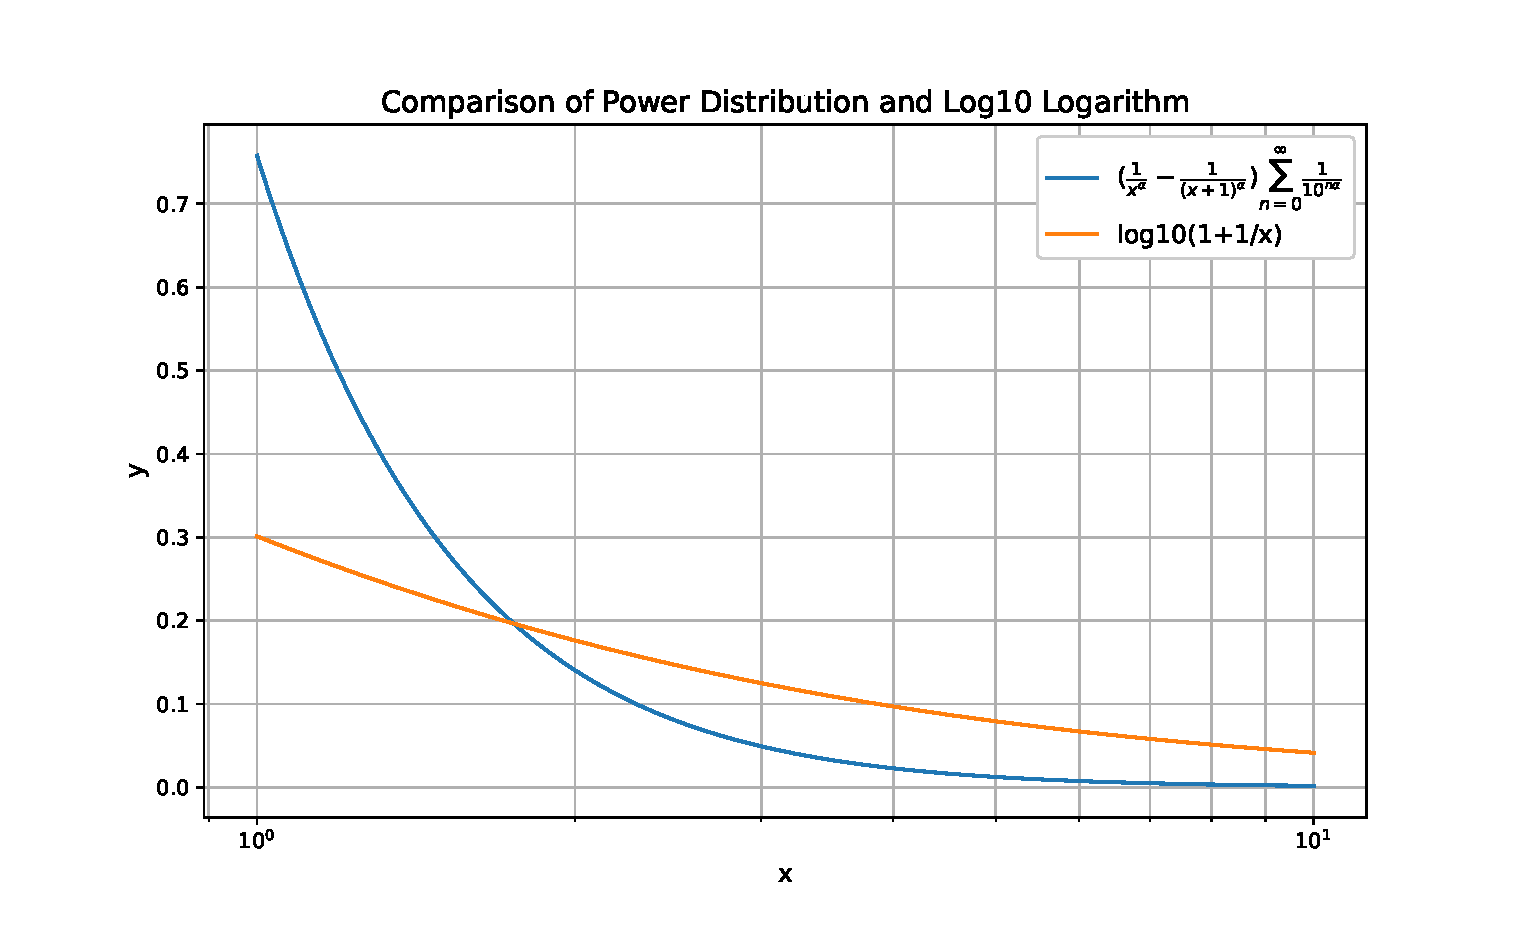
\includegraphics[width=\textwidth]{power2.eps}
        \caption{|$\alpha$|远离1时的幂分布}
    \end{minipage}
\end{figure}

当参数 $ a $ 较小,且幂次 $ \alpha $ 接近于 $ -1 $ 时,幂分布的特征将愈发接近于本福特定律。反之,当幂次 $ |\alpha| $ 增大时,分布的首位数将更倾向于较小的数字,这一趋势愈发显著。这一现象并不令人意外,因为函数 $ B(x) = \log_{10}(x+1) - \log_{10}x $ 在某个区间上与 $ \frac{1}{t} $ 的定积分形式相似。然而,在评估一个分布是否符合本福特定律时,我们并未采用 $ f(t) \approx \frac{1}{t} $ 作为近似标准。原因主要有二:首先,$ \frac{1}{t} $ 的积分在相应区间上是不收敛的;其次,这种估计方法过于粗略,容易导致误判。

\begin{figure}[H]
    \begin{minipage}{0.48\textwidth}
        \includegraphics[width=\textwidth]{norm1.eps}
        \caption{方差较小时的半正态分布}
    \end{minipage}
    \hfill
    \begin{minipage}{0.48\textwidth}
        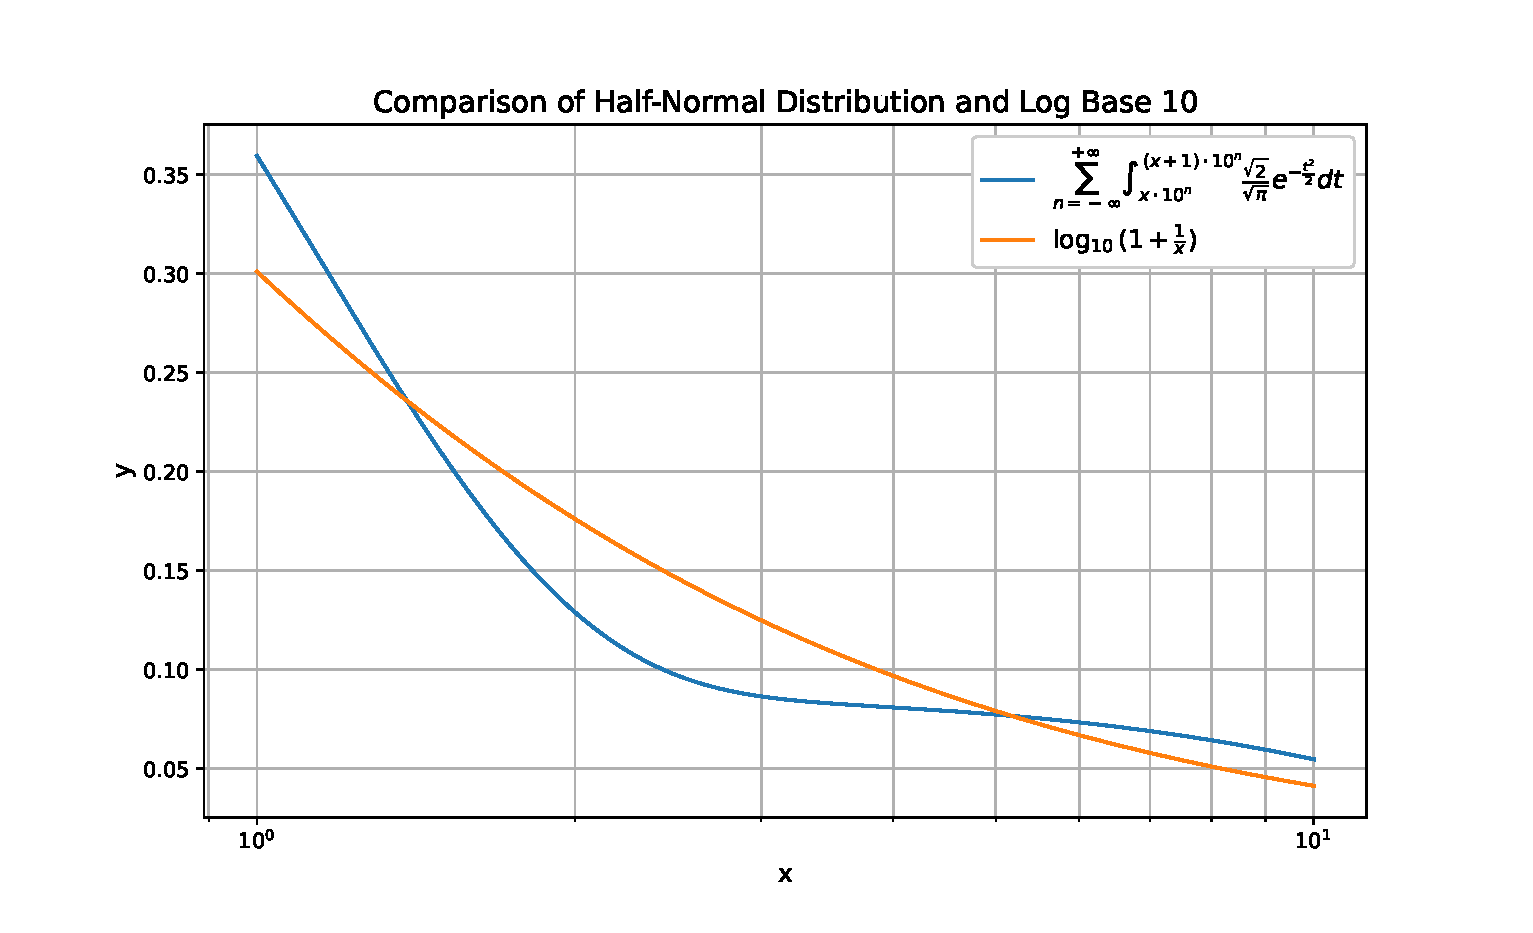
\includegraphics[width=\textwidth]{norm2.eps}
        \caption{方差较大时的半正态分布}
    \end{minipage}
\end{figure}

无论方差是多少,半正态分布都和本福特定律有明显的区别。

事实上,指数分布和对数正态分布二者都是高度符合(10)条件的:

\begin{figure}[H]
    \begin{minipage}{0.48\textwidth}
        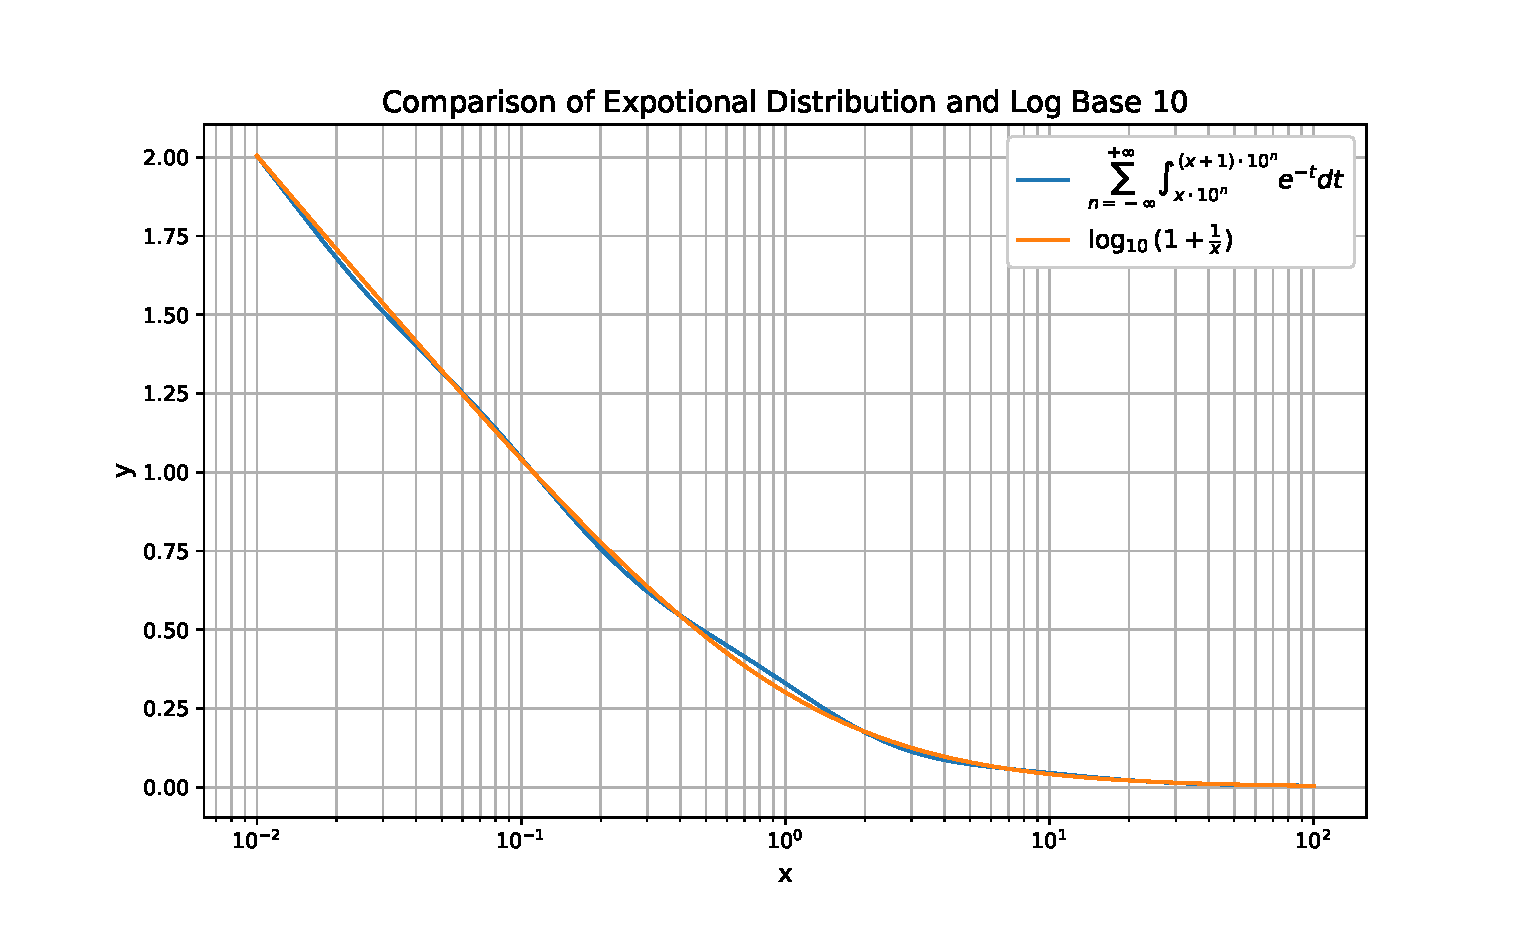
\includegraphics[width=\textwidth]{exp.eps}
        \caption{指数分布与本福特定律的对比(a=1)}
    \end{minipage}
    \hfill
    \begin{minipage}{0.48\textwidth}
        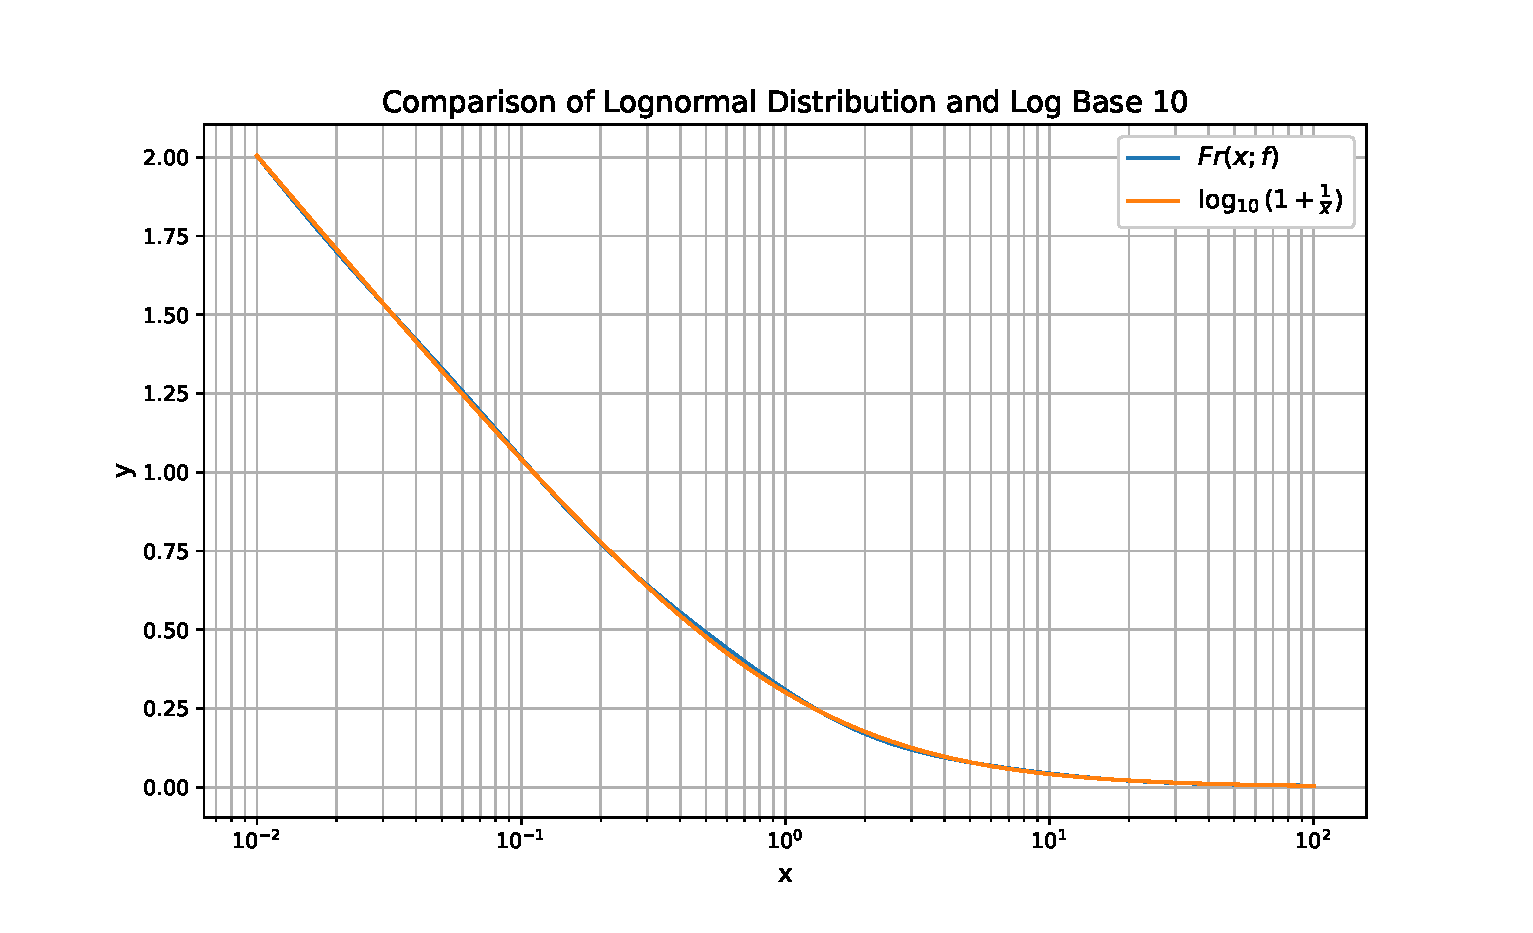
\includegraphics[width=\textwidth]{log.eps}
        \caption{对数正态分布与本福特定律的对比}
    \end{minipage}
\end{figure}

观察到指数分布在很大程度上与本福特定律相符。

我们注意到,除了在 $ b $ 极端小的特定情况下,对数正态分布在一般情况下与本福特定律的符合程度非常高。具体而言,分布的累积分布函数 $ F_r(x; \mu, \sigma) $ 与本福特定律的分布函数 $ B(x) $ 几乎完全一致。值得一提的是,对数正态分布揭示的是乘性增长的中心极限定理,所以我们可以得出乘性增长的数据是符合本福特定律的,但是符合本福特定律的数据是否一定乘性增长还有待商榷。




\section{仿真实验与分析}

\subsection{方差量定义及数据集分析}

我们定义了一个刻画数据集和本福特定律的差别的方差量,并对kaggle上的地外行星周期、人口数据等无人为操控的数据集进行了分析。结果表明,这些数据集符合本福特定律,且具有正偏度和较大的峰度。

\subsection{仿真实验结果}

\begin{itemize}
    \item 当数据集偏度为负时,本福特定律的图像将倒置;
    \item 峰度和方差具有负相关性,峰度较大时数据集更接近本福特分布;
    \item 通过仿真实验,我们找到了一系列符合本福特定律的分布。
\end{itemize}

\section{分析与总结}

\subsection{分析}

通过对本福特定律的研究,我们了解了自然产生数据集的分布特点,以及符合本福特定律的随机变量特性。此外,我们还发现了一些新的符合本福特定律的分布。

\subsection{总结}

本福特定律为揭示自然产生数据集的分布规律提供了有力工具。通过对本福特定律的探究,我们更好地理解了“自然产生(非人为操控)”的定义,并为实际应用提供了理论依据。在今后的研究中,我们可以进一步探讨本福特定律在其他领域的应用,以及如何将其应用于数据造假检测等方面。

\begin{thebibliography}{9}
    \bibitem{wiki_benford}
    "本福特定律," 维基百科. [Online]. Available: \url{https://zh.wikipedia.org/wiki/%E6%9C%AC%E7%A6%8F%E7%89%B9%E5%AE%9A%E5%BE%8B}. [Accessed: \today]
    
    \bibitem{Simon}
    S. Newcomb, "Note on the Frequency of Use of the Different Digits in Natural Numbers," American Journal of Mathematics, vol. 4, no. 1, pp. 39-40, 1881, doi: 10.2307/2369148.

    \bibitem{Hilla}
    T. P. Hill, "A Statistical Derivation of the Significant-Digit Law," Statistical Science, vol. 10, no. 4, pp. 354-363, 1995.

    \bibitem{Hillb}
    T. P. Hill, "Base-invariance implies Benford's law," Proceedings of the American Mathematical Society, vol. 123, pp. 887-895, 1995.

    \bibitem{Kallenberg}
    O. Kallenberg, "Random Measures," New York, NY, USA: Academic Press, 1983.

    \bibitem{Iran}
    "Statistics hint at fraud in Iranian election," New Scientist, Jun. 24, 2009. [Online]. Available: https://www.newscientist.com/article/mg20227144-000-statistics-hint-at-fraud-in-iranian-election/ [Accessed: Dec. 21, 2024].
\end{thebibliography}

\end{document}

